%Example of use of oxmathproblems latex class for problem sheets
\documentclass{oxmathproblems}
\usepackage{tikz}
\usepackage{algorithmic}
\usepackage{algorithm,float}
\usepackage{hyperref}
\hypersetup{hidelinks,
  colorlinks=true,
  allcolors=black,
  pdfstartview=Fit,
  breaklinks=true}

%(un)comment this line to enable/disable output of any solutions in the file
%\printanswers

%define the page header/title info
\course{Algorithm Design and Analysis (Fall 2023)}
\sheettitle{Assignment 3\\Deadline: Dec 12, 2023\\\small{Yuqing Tu 522030910152}} %can leave out if no title per sheet

\begin{document}
\begin{questions}

  \makeatletter
  \newenvironment{breakablealgorithm}
    {% \begin{breakablealgorithm}
    \begin{center}
      \refstepcounter{algorithm}% New algorithm
      \hrule height.8pt depth0pt \kern2pt% \@fs@pre for \@fs@ruled 画线
      \renewcommand{\caption}[2][\relax]{% Make a new \caption
      {\raggedright\textbf{\ALG@name~\thealgorithm} ##2\par}%
      \ifx\relax##1\relax % #1 is \relax
        \addcontentsline{loa}{algorithm}{\protect\numberline{\thealgorithm}##2}%
      \else % #1 is not \relax
        \addcontentsline{loa}{algorithm}{\protect\numberline{\thealgorithm}##1}%
      \fi
      \kern2pt\hrule\kern2pt
      }
    }{% \end{breakablealgorithm}
      \kern2pt\hrule\relax% \@fs@post for \@fs@ruled 画线
    \end{center}
    }
  \makeatother

\miquestion[25]
Given a constant $k\in\mathbb{Z}^+$, we say that a vertex $u$ in an undirected graph \emph{covers} a vertex $v$ if the distance between $u$ and $v$ is at most $k$. In particular, a vertex $u$ covers all those vertices that are within distance $k$ from $u$, including $u$ itself. Given an undirected \emph{tree} $G=(V,E)$ and the parameter $k$, consider the problem of finding a minimum-size subset of vertices that covers all the vertices in $G$.
Design a polynomial time algorithm for this problem. Prove the correctness of your algorithm and analyze its running time.
You will receive 15 points if you can solve the problem for $k=1$.

\textbf{Solution:}

\begin{breakablealgorithm}
  \caption{$set_cover(k, G)$}
  \begin{algorithmic}[1]
    \STATE{$cnt \leftarrow 0$}
    \WHILE{there are some $v \in V$ that are not covered}
    \STATE{find the longest path $p$ in $G$, which is $v_0, v_1, \cdots, v_n$, such that $v_0$ and $v_n$ must not be covered}
    \STATE{choose $v_{v-k}$ as the coverage center}
    \STATE{$++cnt$}
    \ENDWHILE
    \RETURN{$cnt$}
  \end{algorithmic}
\end{breakablealgorithm}

Correctness proof:\\
It is obvious that if the length of the longest path $p$ in $G$ is smaller than or equal to $2k$, we can use one vertex to cover $G$. So we should gradually reduce the length of the longest path.
For the longest path $p$ in $G$, which is $v_0, v_1, \cdots, v_n$, in order to cover $v_n$, we should choose $v_{v-z}$ ($z \leq k$) as the coverage center, and in this greedy algorithm, we choose $v_{v-k}$.
Assume there is a coverage center $v_{n-m}$ ($m < k$). If the set of points $C_{n-m}$ covered by $v_{n-m}$ is a subset of the set of points $C_{n-k}$ covered by $v_{v-k}$, then we can say that the cover of $v_{v-k}$ is better. It means that the greedy algorithm is correct.\\
Now proof it by contradiction. Assume there is a $v \in C_{n-m}$ but $v \notin C_{n-k}$. Then we have $l_{v, v_{n-k}} > k$, where $l_{v, v_{n-k}}$ is the length of the path from $v$ to $v_{n-k}$.
And we know that $l_{v_0, v_{n-k}} = n - k$, then $l_{v_0, v} = l_{v_1, v_{n-k}} + l_{v, v_{n-k}} > n - k + k = n$. So there is a path longer than $p$. There is a contradiction. So the algorithm is correct.

Time complexity:\\
Because $G$ is a tree, so we can run two BFS to find the longest path, which time complexity is $O(|V|+|E|)$. And the loop is executed at most $|V|$ times because in each round we must choose a vertex. So the total time complexity is $O(|V|^2+|V||E|)$, which is polynomial.


\miquestion[25]
Suppose you are a driver, and you plan to drive from $A$ to $B$ through a highway with distance $D$. 
Since your car's tank capacity $C$ is limited, you need to refuel your car at the gas station on the way. 
We are given $n$ gas stations on the highway with surplus supply. 
Let $d_i\in(0,D)$ be the distance between the starting point $A$ and the $i$-th gas station.
Let $p_i$ be the price for each unit of gas at the $i$-th gas station.
Suppose each unit of gas exactly supports one unit of distance. 
The car's tank is empty at the beginning, and the $1$-st gas station is at $A$. 
Design efficient algorithms for the following tasks.
\begin{parts}
    \part[5] Determine whether it is possible to reach $B$ from $A$. 
    \part[20] Minimized the gas cost for reaching $B$. 
\end{parts}  
Please prove the correctness of your algorithms and analyze their running times.

\textbf{Solution:}

\begin{parts}
    \part If there exists an $i$ and $d_{i+1} - d_i > C$, then it is impossible to reach $B$ from $A$.
    If $d_{i+1} - d_i \leq C$ for every $i$, then it is possible to reach $B$ from $A$.

    Correctness proof:\\
    If we just want to reach $B$, there is a stupid algorithm that we fill up the tank at every gas station.
    So if there exists an $i$ and $d_{i+1} - d_i > C$, even the tank is full, we must not be able to reach to the $i$-th gas station.
    And if $d_{i+1} - d_i \leq C$ for every $i$, because when we left the $i$-th gas station, the tank is full, so we must be able to reach to the next gas station.

    Time complexity:\\
    This algorithm just traverses $d[1\cdots n]$, so the time complexity is $O(n)$.
    \part 
    \begin{breakablealgorithm}
    \caption{$min\_cost(C, D, d[1\cdots n], p[1\cdots n])$}
    \begin{algorithmic}[1]
      \STATE{$d[n+1] \leftarrow D$, $p[n+1] \leftarrow 0$}
      \STATE{$pos \leftarrow 1$, $cost \leftarrow 0$, $V \leftarrow 0$}
      \WHILE{$pos \leq n$}
      \IF{There is at least one $i$, such that $d_i - d_{pos} \leq C$ and $p_i \leq p_{pos}$}
      \STATE{Find the smallest $i$}
      \STATE$cost \leftarrow cost + p_{pos} * (d_i - d_{pos} - V)$, {$V \leftarrow d_i - d_{pos}$}
      \STATE{$V \leftarrow V - (d_i - d_{pos})$, $pos \leftarrow i$}
      \ELSE
      \STATE{$cost \leftarrow cost + p_{pos} * (C - V)$, $V \leftarrow C$}
      \STATE{$V \leftarrow V - (d_{pos+1} - d_{pos})$, $pos \leftarrow pos + 1$}
      \ENDIF
      \ENDWHILE
      \RETURN{$cost$}
    \end{algorithmic}
    \end{breakablealgorithm}
    \end{parts}
    Correctness proof:\\
    Prove by contradiction. Assume that we refuel less or more gas in gas stations.
    \begin{itemize}
      \item [1)] If we refuel less gas:\\
      If there is the nearest and reachable gas station whose price is lower than the station we're at now, then we can't reach to it.
      So we need more cost to reach this station (we must refuel more expensive gas at the station halfway through) or even can't reach to it (there is not any station halfway through).
      It is definitely not a part of the optimal solution.\\
      If all reachable stations' price is higher than the station we're at now, then when we reach at the next station, we'll have less gas left or none at all.
      So we need more cost to refuel next time because we left less cheaper gas.
      It is also definitely not a part of the optimal solution.
      \item [2)] If we refuel more gas:\\
      If there is the nearest and reachable gas station whose price is lower than the station we're at now, then when we reach at the next station, we'll still have some more expensive gas left.
      So we can only buy less cheaper gas.
      It is definitely not a part of the optimal solution.\\
      If all reachable stations' price is higher than the station we're at now. This case is unlikely to happen because we can't overfill the tank.
    \end{itemize}
    To sum up, if we refuel less or more gas, we can't get a part of the optimal solution. So the algorithm is correct.

    Time complexity:\\
    Assuming a worst case: t he price at the gas stations is increasing. Then there are $n$ times loops. In each loop, at most $n$ comparisons will be made. So the time complexity is $O(n^2)$.

\miquestion[25]
  Given a ground set $U=\{1,\ldots,n\}$, a \emph{set function on $U$} is a function $f:\{0,1\}^U\to\mathbb{R}$ that maps a subset of $U$ to a real value.
  A set function $f$ is \emph{submodular} if
  $$f(S\cup\{v\})-f(S)\geq f(T\cup\{v\})-f(T)$$
  holds for any $S,T\subseteq U$ with $S\subseteq T$ and any $v\in U\setminus T$.
  We make the following assumptions on a submodular set function $f$:
  \begin{itemize}
    \item Nonnegative: $f(S)\geq0$ for any $S\subseteq U$; you can assume $f(S)$ is always a rational number.
    \item Monotone: $f(S)\leq f(T)$ for any $S,T\subseteq U$ with $S\subseteq T$.
    \item $f(S)$ can be computed in a polynomial time with respect to $n=|U|$.
  \end{itemize}
  Given a positive integer $k>0$ as an input, the goal is to find $S\subseteq U$ that maximizes $f(S)$ subject to the cardinality constraint $|S|\leq k$.
  Design a polynomial time $(1-1/e)$-approximation algorithm for this maximization problem.
  Prove that the algorithm you design runs in a polynomial time and provides a $(1-1/e)$-approximation.
  
  \textbf{Solution:}

  \begin{breakablealgorithm}
  \caption{$max\_f(k, U)$}
  \begin{algorithmic}[1]
    \STATE{$S \leftarrow \emptyset$}
    \FOR{$k$ rounds}
    \STATE{find $A \in U \verb|\| S$ that maximizes $f(S \cup \{A\}) - f(S)$}
    \STATE{$S \leftarrow S \cup \{A\}$}
    \ENDFOR
    \RETURN{$S$}
  \end{algorithmic}
  \end{breakablealgorithm}

  Time complexity:\\
  In this algorithm, we do $k$ rounds. And in each round, we traverses $U \verb|\| S$ to find the set $A$ we need, whose time complexity is $O(n)$, and each calculation of $f$'s time complexity is $O(n^m)$ ($m$ is one canstant positive integer).
  So the total time complexity is $O(kn^{m+1})$.

  Approximation proof:\\
  First, we should prove a lemma:\\
  Let $S_l = \{A_1, A_2, \cdots, A_l\}$ be the output of this algorithm after $l$ iterations, and $S^* = \{O_1, O_2, \cdots, O_k\}$ be any collection of $k$ subsets.
  $$f(S_l) \geq \left(1-\left( 1-\frac{1}{k} \right)^l \right)f(S^*)$$
  Prove by induction.\\
  \begin{itemize}
      \item Base step: $l = 1$
      \item By greedy nature, $f(S_1) \geq f(\{O_i\})$ for all $O_i$
      \item Thus, $f(S_1) \geq \frac{1}{k}\sum_{i = 1}^{k}f(\{O_i\}) \geq \frac{1}{k}f(S^*) = \left(1-\left( 1-\frac{1}{k} \right)^1 \right)f(S^*)$
      \item Middle inequality:\\
      $\because f(S\cup\{v\})-f(S)\geq f(T\cup\{v\})-f(T)$\\
      $\therefore f(\{v\})-f(\emptyset)\geq f(T\cup\{v\})-f(T)$\\
      $\therefore f(\{v\})+f(T)\geq f(T\cup\{v\})$
      \item Inductive step: suppose $f(S_t) \geq \left(1-\left( 1-\frac{1}{k} \right)^t \right)f(S^*)$
      \item By greedy nature,
    \begin{align}
      f(S_{t+1}) - f(S_t) &\geq \frac{1}{k} \sum_{i = 1}^{k}  f(S_t\cup\{O_i\}) - f(S_t) \notag\\
                          &\geq \frac{1}{k} [f(S_t \cup S^*) - f(S_t)] \notag\\
                          &\geq \frac{1}{k} [f(S^*) - f(S_t)] \notag
    \end{align}
    \begin{align}
    f(S_{t+1}) &\geq \frac{1}{k} f(S^*) + \left( 1 - \frac{1}{k} \right)f(S_t) \notag\\
               &\geq \frac{1}{k}f(S^*) + \left( 1 - \frac{1}{k} \right)\left(1-\left( 1-\frac{1}{k} \right)^t \right)f(S^*) \notag\\
               &= \left(1-\left(1-\frac{1}{k}\right)^{t+1}\right)f(S^*) \notag
    \end{align}
    \item The lemma is proved.
  \end{itemize}
  In this algorithm, we do $k$ iterations, so $l = k$. We have $f(S) \geq \left(1-\left( 1-\frac{1}{k} \right)^k \right)f(S^*) \geq \left(1-\frac{1}{e}\right)f(S^*)$.
  So this algorithm provides a $\left(1-\frac{1}{e}\right)$-approximation.

\miquestion[25]
Given an undirected graph $G=(V,E)$, a \emph{matching} $M$ is a subset of edges such that no two edges in $M$ share an endpoint.
The \emph{maximum matching problem} takes the graph $G=(V,E)$ as the input and outputs a matching $M$ with the maximum size $|M|$.
Consider the following greedy algorithm.
\begin{itemize}
    \item initialize $M\leftarrow\emptyset$\;
    \item while there exists $e\in E$ such that $M\cup\{e\}$ is a valid matching:
    \begin{itemize}
        \item update $M\leftarrow M\cup\{e\}$\;
    \end{itemize}
    \item endwhile
    \item return $S$\;
\end{itemize}
\begin{parts}
    \part[20] Prove that this is a $0.5$-approximation algorithm.
    \part[5] Provide a tight example showing that this is not a $(0.5+\varepsilon)$-approximation algorithm for any $\varepsilon>0$.
\end{parts}

\textbf{Solution:}

\begin{parts}
  \part For this algorithm, suppose the approximation ratio is $\alpha$. Assume that the optimal solution is $M_{opt}$ and the greed solution is $M$.\\
  First, assume $G$ is a connected graph. For any adjacent $e_{1, 2} \in M/M_{opt}$, there are one or two edges that not in $M/M_{opt}$ between them.
  So for the maximum $|M_{opt}|$, there is only one edge that not in $M_{opt}$ between all adjacent $e_{1, 2} \in M/M_{opt}$. Then the maximum $|M_{opt}| = \lceil \frac{|E|}{2} \rceil $.
  And for the minimum $|M|$, there are only two edge that not in $M$ between all adjacent $e_{1, 2} \in M$. Then the minimum $|M| = \lceil \frac{|E|}{3} \rceil $.
  So the lower bound of the approximation ratio $\alpha = \min \left\{\frac{\lceil \frac{|E|}{3} \rceil}{\lceil \frac{|E|}{2} \rceil}\right\} = 0.5$.\\
  Second, for the unconnected graph $G$, its each connected component satisfies the approximation ratio of $0.5$, then the total approximation ratio, which is the weighted average of approximation ratios for each connected component, is also $0.5$.
  \part The red edges are selected by this algorithm.

  A optimal solution:
  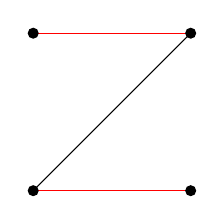
\begin{tikzpicture}
    \draw[red] (0,0) -- (2,0);
    \draw[red] (0,2) -- (2,2);
    \draw (0,0) -- (2,2);
    \fill (0,0) circle (2pt);
    \fill (2,0) circle (2pt);
    \fill (2,2) circle (2pt);
    \fill (0,2) circle (2pt);
  \end{tikzpicture}
  \ \ \ The worst solution:
  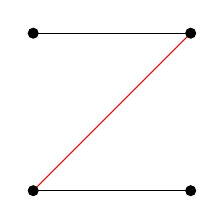
\begin{tikzpicture}
    \draw (0,0) -- (2,0);
    \draw (0,2) -- (2,2);
    \draw[red] (0,0) -- (2,2);
    \fill (0,0) circle (2pt);
    \fill (2,0) circle (2pt);
    \fill (2,2) circle (2pt);
    \fill (0,2) circle (2pt);
  \end{tikzpicture}\\
  In this case, the approximation ratio $\alpha = \frac{1}{2} = 0.5$, so there is not a $(0.5+\varepsilon)$-approximation algorithm for any $\varepsilon>0$.
\end{parts}

\miquestion
How long does it take you to finish the assignment (including thinking and discussion)?
Give a score (1,2,3,4,5) to the difficulty.
Do you have any collaborators?
Please write down their names here.

I can't exactly say how much time I spent. During the week, I thought about this assignment on and off. And I spent about $2$ hours to write down my ideas.
I'll give a 5 to the difficulty. This assignment is really difficult.

\end{questions}
\end{document}
